\chapter{Foundations}\label{chapter_Foundations}
This chapter provides conceptual foundations that are essential for understanding the development process of the editor. First, the basics of model-driven software development (MDSD) important in this context are presented, followed by an exploration of the SCCharts language.
\section{Model-Driven Software Development}\label{Model-Driven Software Development}
Before clarifying what exactly MDSD is, the term model must be defined more precisely.

\subsection{Model}
Generally a model can be said to serve as a simplified or partial representation of real entities, designed to emphasise essential information or features while omitting less important details. Models are used in many fields, from science to business, and serve as valuable tools to understand, analyse and communicate complicated phenomena or processes. In the realm of software engineering, models assume diverse roles, spanning from describing systems or the specification of requirements to the generation of configuration files or executable code based on the information encapsulated within these models.~\cite{Brambilla.2017}

\subsection{Goals of Model-Driven Software Development}
First of all, it should be clarified what is meant by MDSD. According to Brambilla et al.~\cite{Brambilla.2017}, MDSD "is a development paradigm that uses models as the primary artifact of the development process. Usually, in [MDSD] the implementation is (semi)automatically generated from the models." The aim is to use models as development artefacts and to use abstraction to hide the unimportant details and highlight the important ones. In addition, it tries to automate as much of the development process as possible. This can start with the definition of requirements and reach up to the final developed software system.

\subsection{Modeling Language}
Modeling languages are an important part in the MDSD. They serve as a mechanism through which designers can articulate both the structure and behavior of their systems, utilizing either graphical or textual representations. Designers are required to adhere to the specific syntax defined by the modeling language they are using. There are two primary classes of modeling languages: GPMLs and DSLs. DSLs are modeling languages designed for a specific domain or area of application. This specialization ease the process of creating models within that particular domain. Conversely, GPMLs can be applied to a wide range of applications but lack the tailored focus found in DSLs.~\cite{Brambilla.2017}

\subsection{Metamodeling}
The term metamodeling describes a concept for creating models from models. The model that is used to create another model is called a metamodel. Thus, a metamodel is essentially a model that describes the structure and semantic rules for a particular class of models. It is used to define the syntax and semantics of a modeling language and to ensure that models created in that language conform to the defined rules. 

A suitable example for this can be seen in Fig. \ref{fig:Meta-Modeling}. When describing real objects through models, the model level M1 defines the syntax and semantics of the level below it, M0. The same applies to the model level in relation to the metamodel level M2. For the metamodel level M2, once again, the syntax and semantics can be defined in the level above it, the meta-metamodel level. This process could continue indefinitely, so that starting from the meta-metamodel level, each subsequent meta-metamodel instance refers to another meta-metamodel instance.~\cite{Brambilla.2017}
\begin{figure}[h!]
\centering
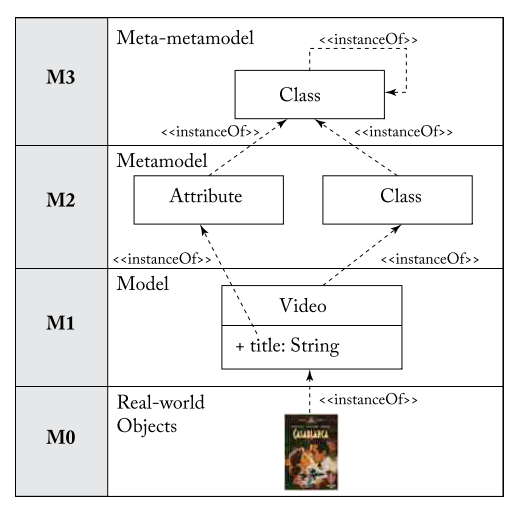
\includegraphics[width=0.7\textwidth]{bilder/Meta-Modeling.png}
\caption{Models, metamodels, and meta-metamodels (from~\cite{Brambilla.2017})}
\label{fig:Meta-Modeling}
\end{figure} 

This example can also be mapped to the creation of a DSL tool for SCCharts. In M3 is the \textsc{Cinco} meta tool with which a DSL tool for SCCharts is to be created (layer M2). This can then be used to create SCCharts models (M1) that represent a SCChart of the SCCharts language (M0).

\section{Sequentially Constructive Statecharts} \label{Sequentially_Constructive_Statecharts}
The visual modeling language SCCharts, which is based on Harel's Statecharts~\cite{Harel.1987}, was designed for safety-critical applications and aim for easy adaptation. It utilize the visual syntax from Charles André's SyncCharts~\cite{andre.} and provides deterministic concurrency based on a synchronous Model of Computation. 

To gain a better understanding of the different elements of the SCCharts syntax, Fig \ref{fig:SCChart-Overview} is helpful. The upper part of depicts the Core-SCCharts, which include concurrency and hierarchy as essential features of Statecharts. While the lower part contains elements of the Extended SCCharts. It should be noted that each advanced feature can be expressed as one or more core features, but the use of advanced features reduces the complexity of the diagram and therefore improves clarity.~\cite{Hanxleden.2014} The components are explained in more detail below.

\begin{figure}[h!]
\centering
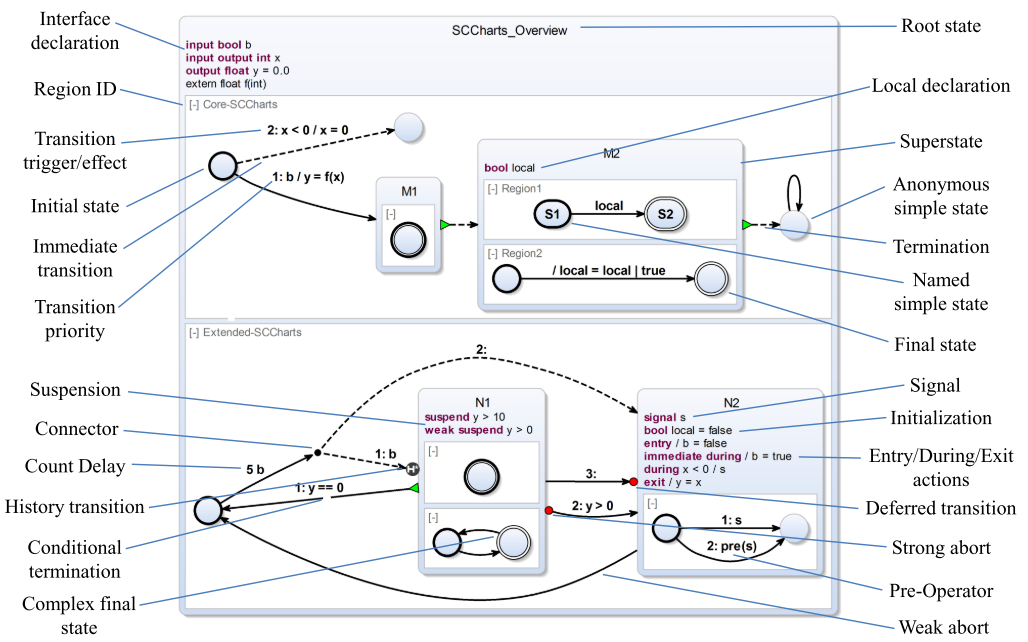
\includegraphics[width=1.0\textwidth]{bilder/SCChart-Overview.png}
\caption{SCCharts-Overview (from~\cite{Hanxleden.2014})}
\label{fig:SCChart-Overview}
\end{figure} 

\subsection{States and SuperStates}
States are a fundamental part of SCCharts. A distinction is made between simple states and states with internal behaviour, so-called superstates. Both types of states can function as initial states (thick border), final states (double border) or initial final states (thick border and double border). Each SCChart also has exactly one root state that behaves like a superstate and in which all behaviour of the SCChart is defined. Additionally, there are connectors (large black dot), which are essentially simple states with the purpose of connecting multiple states through outgoing and incoming edges.
\subsection{Transitions}
Another basic component is transitions. Each transition has a source state and a target state. Transitions can have a label with the syntax \textit{[p:] [t] [/ a]}, where p stands for priority, t for trigger and a for action. The trigger is a side-effect-free boolean expression and the action is an assignment of any data type. A state is said to be active when the SCChart is in that particular state. If the source state of a transition is active and the trigger becomes true, the target state is active. The transition can be immediate (dashed transition) or delayed. Immediate means that the state becomes active on the same tick (stimulus), while delayed means that the state becomes active on the next tick. Transitions are delayed by default to avoid causality problems. The priority is used to check the trigger in ascending order, so that if there are, for example, two transitions with true triggers, the one with the higher priority is used.~\cite{Motika.2017}
\subsection{Declarations}
Declarations of variables can be made at the top of any superstate, including root states. These variables can be inputs, which are read from the environment, or outputs, which are written to the environment. Additionally, they can also be input output variables or local variables, which are used only internally. The data types for these variables can include boolean, integer, float, and string. Local variables can also be uninitialized or pre-assigned, and their values persist even when, for example, the superstate where they are defined is exited. Furthermore, there are signals used for communication with the environment and among the components of the SCChart. Pure signals are interpreted as boolean values and are true when present and false when absent. In contrast, valued signals carry a typed value in addition to their presence status. Lastly, declarations can be marked as constant, which means that the value cannot be changed after initialization.~\cite{Motika.2017}
\subsection{Hierarchy and Concurrency}
Superstates, including the root state, have inner behavior, which includes one or several concurrent regions (represented by white boxes). Each region conceptually corresponds to a thread, and each region must contain an initial state. If a final state is entered within a region, that region terminates. Termination transitions (green triangle at the source state) can originate from superstates and are taken when all regions within the superstate are in final states. These transitions are typically unconditional, and superstates usually have only one of them. If there are multiple termination transitions, the one with the highest priority is taken.~\cite{Motika.2017}

\subsection{Actions and Suspensions}

Actions and suspensions are specified beneath the declarations of superstates. There are four distinct types of actions that influence the behavior of the associated superstate. These actions have an effect and may include an optional condition. Entry and exit actions are executed when entering or exiting the superstate, either when they have no condition or when their optional condition evaluates to true. Additionally, there are during and immediate during actions, which are executed if the superstate they are associated with is active and they either have no condition or a condition that evaluates to true. Depending on their type, they may be executed with a delay or immediately.~\cite{Motika.2017}

Suspensions suppress the inner behavior of a superstate, if their trigger is evaluated to true. Their also four different types. Immediate and delayed suspensions are self-explanatory. Weak suspensions and immediate weak suspensions allows immediate inner behavior of a suspensions state but the weakly suspended state remains in the exact same internal states.~\cite{Motika.2017}

\subsection{Complex Transitions}
Beyond the simple transitions described initially, there are additional transitions that have effects upon entering or exiting superstates. One of these is history transition (H at the target state), which allows the execution to continue in the state that was active when the superstate was left. Shallow history applies only to the top level of the superstate, while deep history (H with *) reaches into the deeper levels as well. Furthermore, there are deferred transitions (red dot at the target state), which preempt all immediate behavior in the target state. Finally, there are strong abort transitions (red dot at the source state). Unlike weak aborts (default transitions), which allow the inner behavior of superstates to continue during the tick, strong aborts terminate them directly.
Additionally, transitions can have a count delay. This means that the condition must be true for a specific number of ticks before the transition is triggered.~\cite{Motika.2017}

\subsection{References}
Another feature of SCCharts is their ability to reference each other. To achieve this, the corresponding inputs and outputs of the referenced SCChart must be assigned variables of the appropriate type. These references then become superstates within the inner behavior of the referenced SCChart. Figure \ref{fig:Beep-Reference} illustrates an example of such a reference. Here, Beep is referenced as a superstate within the region of Root. In this case, the input boolean second from Root is assigned to the input second of Beep, and the output boolean speaker from Root is assigned to the output boolean beep of Beep.
\begin{figure}[h!]
\centering
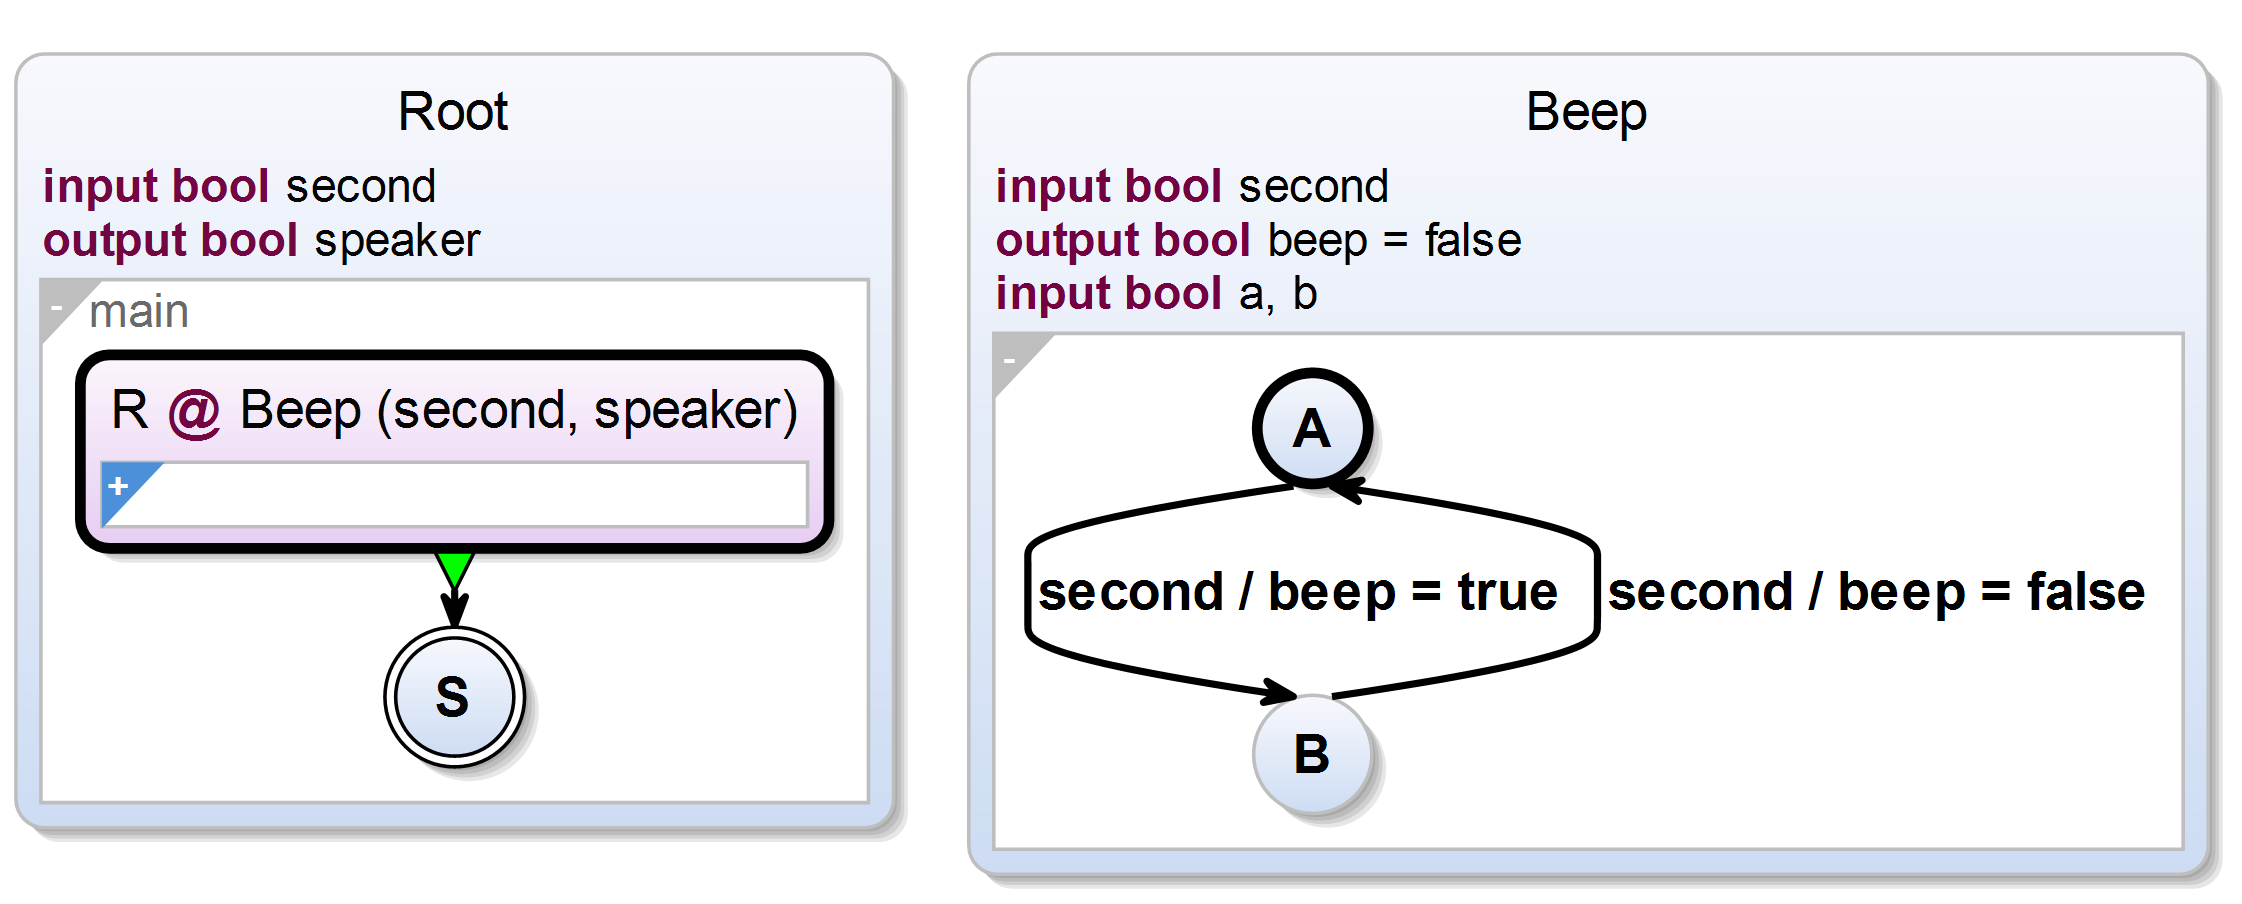
\includegraphics[width=1.0\textwidth]{bilder/BEEP_Reference_Example.png}
\caption{Beep Example for references in SCCharts (adapted from~\cite{.04.09.2023})}
\label{fig:Beep-Reference}
\end{figure} 

